\iffalse
\documentclass[12pt]{article}
\usepackage{graphicx}
\usepackage[none]{hyphenat}
\usepackage{graphicx}
\usepackage{listings}
\usepackage[english]{babel}
\usepackage{graphicx}
\usepackage{caption} 
\usepackage{booktabs}
\usepackage{array}
\usepackage{amssymb} % for \because
\usepackage{amsmath}   % for having text in math mode
\usepackage{extarrows} % for Row operations arrows
\usepackage{listings}
\lstset{
  frame=single,
  breaklines=true
}
\usepackage{hyperref}
  
%Following 2 lines were added to remove the blank page at the beginning
\usepackage{atbegshi}% http://ctan.org/pkg/atbegshi
\AtBeginDocument{\AtBeginShipoutNext{\AtBeginShipoutDiscard}}


%New macro definitions
\newcommand{\mydet}[1]{\ensuremath{\begin{vmatrix}#1\end{vmatrix}}}
\providecommand{\brak}[1]{\ensuremath{\left(#1\right)}}
\providecommand{\norm}[1]{\left\lVert#1\right\rVert}
\providecommand{\abs}[1]{\left\vert#1\right\vert}
\newcommand{\solution}{\noindent \textbf{Solution: }}
\newcommand{\myvec}[1]{\ensuremath{\begin{pmatrix}#1\end{pmatrix}}}
\let\vec\mathbf


\begin{document}

\begin{center}
\title{\textbf{Conic Sections - Hyperbola}}
\date{\vspace{-5ex}} %Not to print date automatically
\maketitle
\end{center}
\setcounter{page}{1}

\section{11$^{th}$ Maths - Chapter 11}
This is Problem-1 from Exercise 11.4
\begin{enumerate}
\solution 
From the given equation of hyperbola, we can get values of
\begin{align}
    a = 4 \\
    b = 3
\end{align}
The given equation of the hyperbola can be rearranged as
\begin{align}
    \label{eq:11/11/4/1hyperEq1}
    9x^2 - 16y^2-144 = 0 
\end{align}
\fi
The given equation can be equated to the generic equation of conic sections
\iffalse
\begin{align}
	\label{eq:11/11/4/1hyperEq2}
	g\brak{\vec{x}} = \vec{x}^T\vec{V}\vec{x} + 2\vec{u}^T\vec{x} + f = 0 
\end{align}
Comparing coefficients of both equations \eqref{eq:11/11/4/1hyperEq1} and \eqref{eq:11/11/4/1hyperEq2} 
\fi
a
\begin{align}
	\label{eq:11/11/4/1eqV}
	\vec{V} &= \myvec{ 9 & 0 \\ 0 & -16} \\
	\label{eq:11/11/4/1eqU}
	\vec{u} &=  0 \\
	\label{eq:11/11/4/1eqF}
	f &= -144 
\end{align}
From equation \eqref{eq:11/11/4/1eqV}, since $\vec{V}$ is already diagonalized, the Eigen values $\lambda_1$ and $\lambda_2$ are given as 
\begin{align}
	\label{eq:11/11/4/1eqEigen1}
	\lambda_1 &= 9 \\
	\label{eq:11/11/4/1eqEigen2}
	\lambda_2 &= -16 
\end{align}
\begin{enumerate}
\item The eccentricity of the hyperbola is given as  
\begin{align}
	e &= \sqrt{1-\frac{\lambda_1}{\lambda_2}} \\
	  &= \sqrt{1-\frac{9}{-16}} \\
          &= \frac{5}{4}
\end{align}
\item For the standard hyperbola, the coordinates of Focii are given as: 
\begin{align}
	\label{eq:11/11/4/1eqFocus}
	\vec{F} &= \pm \frac{\brak{\frac{1}{e\sqrt{1-e^2}}}\brak{e^2}\sqrt{\frac{\lambda_2}{f_0}}}{\frac{\lambda_2}{f_0}}\vec{e1} 
\end{align}
where
\begin{align}
	f_0 &= -f \\
	\eqref{eq:11/11/4/1eqFocus} \implies &=  \pm \frac{\brak{\frac{1}{\frac{5}{4}\sqrt{1-\frac{25}{16}}}}\brak{\frac{25}{16}}\sqrt{\frac{-16}{144}}\vec{e_1}}{\frac{-16}{144}} \\
	&= \pm \myvec{5 \\ 0}
\end{align}
\item The vertices of the hyperbola are given by 
\begin{align}
	& \pm\myvec{ a \\ 0} \\
	&= \pm\myvec{4 \\ 0}
\end{align}
\item The length of the latus rectum is given as 
\begin{align}
	\label{eq:11/11/4/1eqLatRectLen}
	& 2\frac{\sqrt{\abs{f_0\lambda_1}}}{\lambda_2} \\
	&= 2\frac{\sqrt{\abs{144\brak{9}}}}{-16} \\
	&= \frac{9}{2}
\end{align}
as length can't be negative. 
The relevant diagram is shown in Figure \ref{fig:11/11/4/1Fig1}
\begin{figure}[!h]
	\begin{center}
		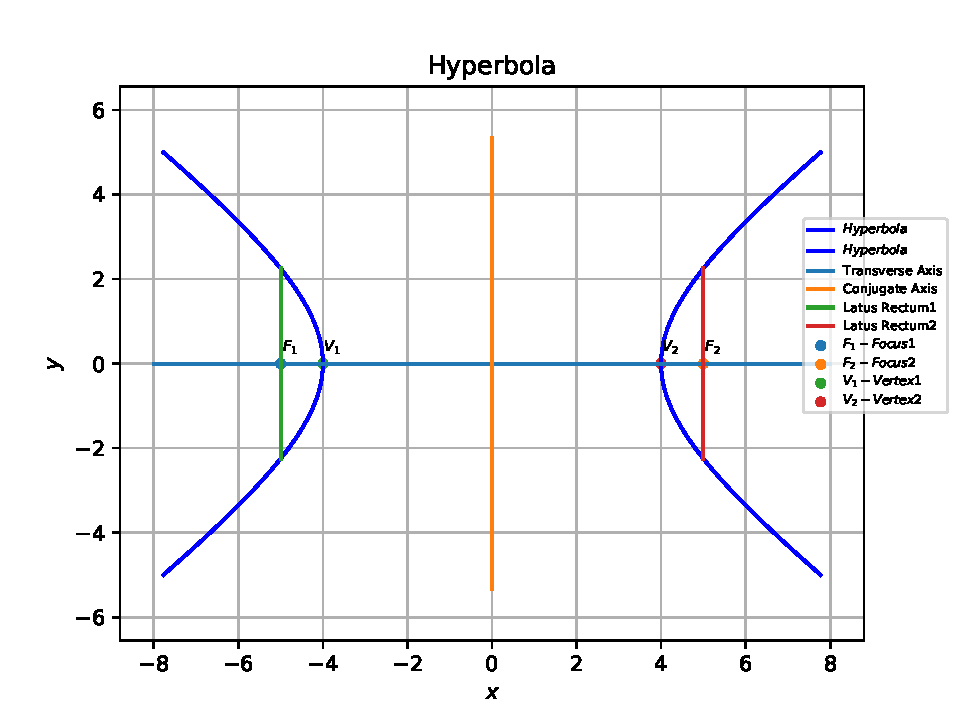
\includegraphics[width=\columnwidth]{chapters/11/11/4/1/figs/problem1.pdf}
	\end{center}
\caption{}
\label{fig:11/11/4/1Fig1}
\end{figure}
\end{enumerate}
